\documentclass[border=4pt,12pt]{standalone}
\usepackage{times}
\usepackage{amsmath,amssymb}
\usepackage{tikz}
\usetikzlibrary{arrows.meta, positioning}
\begin{document}
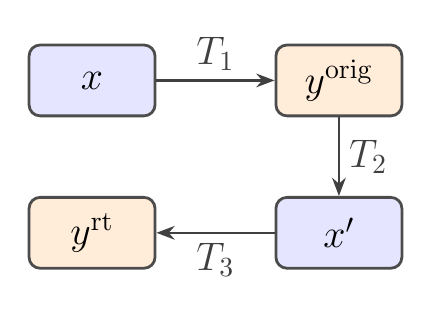
\begin{tikzpicture}[>=Stealth, font=\Large, node distance=1.0cm and 1.5cm,
  box/.style={draw=black!70, rounded corners=4pt, minimum width=1.6cm, minimum height=0.9cm, line width=1pt},
  nl/.style={box, fill=blue!10}, fm/.style={box, fill=orange!15}]
\node[nl] (x) {$x$};
\node[fm, right=of x] (y) {$y^{\mathrm{orig}}$};
\node[nl, below=of y] (xp) {$x'$};
\node[fm, below=of x] (yrt) {$y^{\mathrm{rt}}$};
\draw[->, thick, black!75] (x) -- node[above] {$T_1$} (y);
\draw[->, thick, black!75] (y) -- node[right] {$T_2$} (xp);
\draw[->, thick, black!75] (xp) -- node[below] {$T_3$} (yrt);
\end{tikzpicture}
\end{document}
